%!TEX root = ../../Bachelorarbeit.tex
\appendixChapter{Anhang}
\label{app:anhang}

\section{Quelltext Beispiel JSON Transformation und Validierung}
\lstinputlisting[caption=Beispiel für Play JSON -Transformation bzw. -Validierung, label=app:jsonbsp, language=scala]{code/json_example.scala}

%--------------------------------------------------------------------------------------------------------------------------------------------

\section{Interview 22.11.2012 - Claudia Nikolai }
\label{sec:interview_nikolai}
Claudia Nikolai ist XXXX der D-School.

\subsection*{Zuständigkeiten}
\label{zustaendigkeiten}

\begin{itemize}
\item inhaltliche Programmgestaltung
\item internationale Kooperation
\item Kontakt zu Kunden
\item Ausbildung der Teacher
\item Teacher (an allen Tagen)
\end{itemize}

\subsection*{Austausch mit anderen Teachern}
\label{austauschmitanderenteachern}

\begin{itemize}
\item Teachermeeting
\item e-mail (Verteiler, Informationen fuer viele Personen)
\item Dropbox\slash Email fuer Content
\end{itemize}

\subsection*{Incom}
\label{incom}

\begin{itemize}
\item space noch nicht privat\slash sichtbar (kein Austausch von vertraulichen Informationen)
\item zu viele Notifications (liest aber alle)
\item nutzt es um Hinweise an andere Teams zu geben
\item sichtet Material an Tagen an denen keine Dschool ist
\end{itemize}

\subsection*{Wichtig fuer die Dokumentation}
\label{wichtigfuerdiedokumentation}

\begin{itemize}
\item Wie haben die Studenten Empathie bekommen? (Wie und wann haben sie sich in den User hineinvesetzt?)
\item Zitate
\item Dokumentation der Phasen
\item welche Methode wurde verwendet und wie gut hat sie funktioniert? -> Evaluierung des DS-Prozesses
\end{itemize}

\subsection*{Wunschsystem}
\label{wunschsystem}

\begin{itemize}
\item System sollte einfach verstaendlich sein, Nutzer haben nur 6--12 Wochen um damit klar zu kommen
\item System muss keine eierlegende Wollmilchsau sein
\end{itemize}

%--------------------------------------------------------------------------------------------------------------------------------------------

\section{Datenmodell von Project-Zoom}
\begin{figure}[h]  
  \centering     
  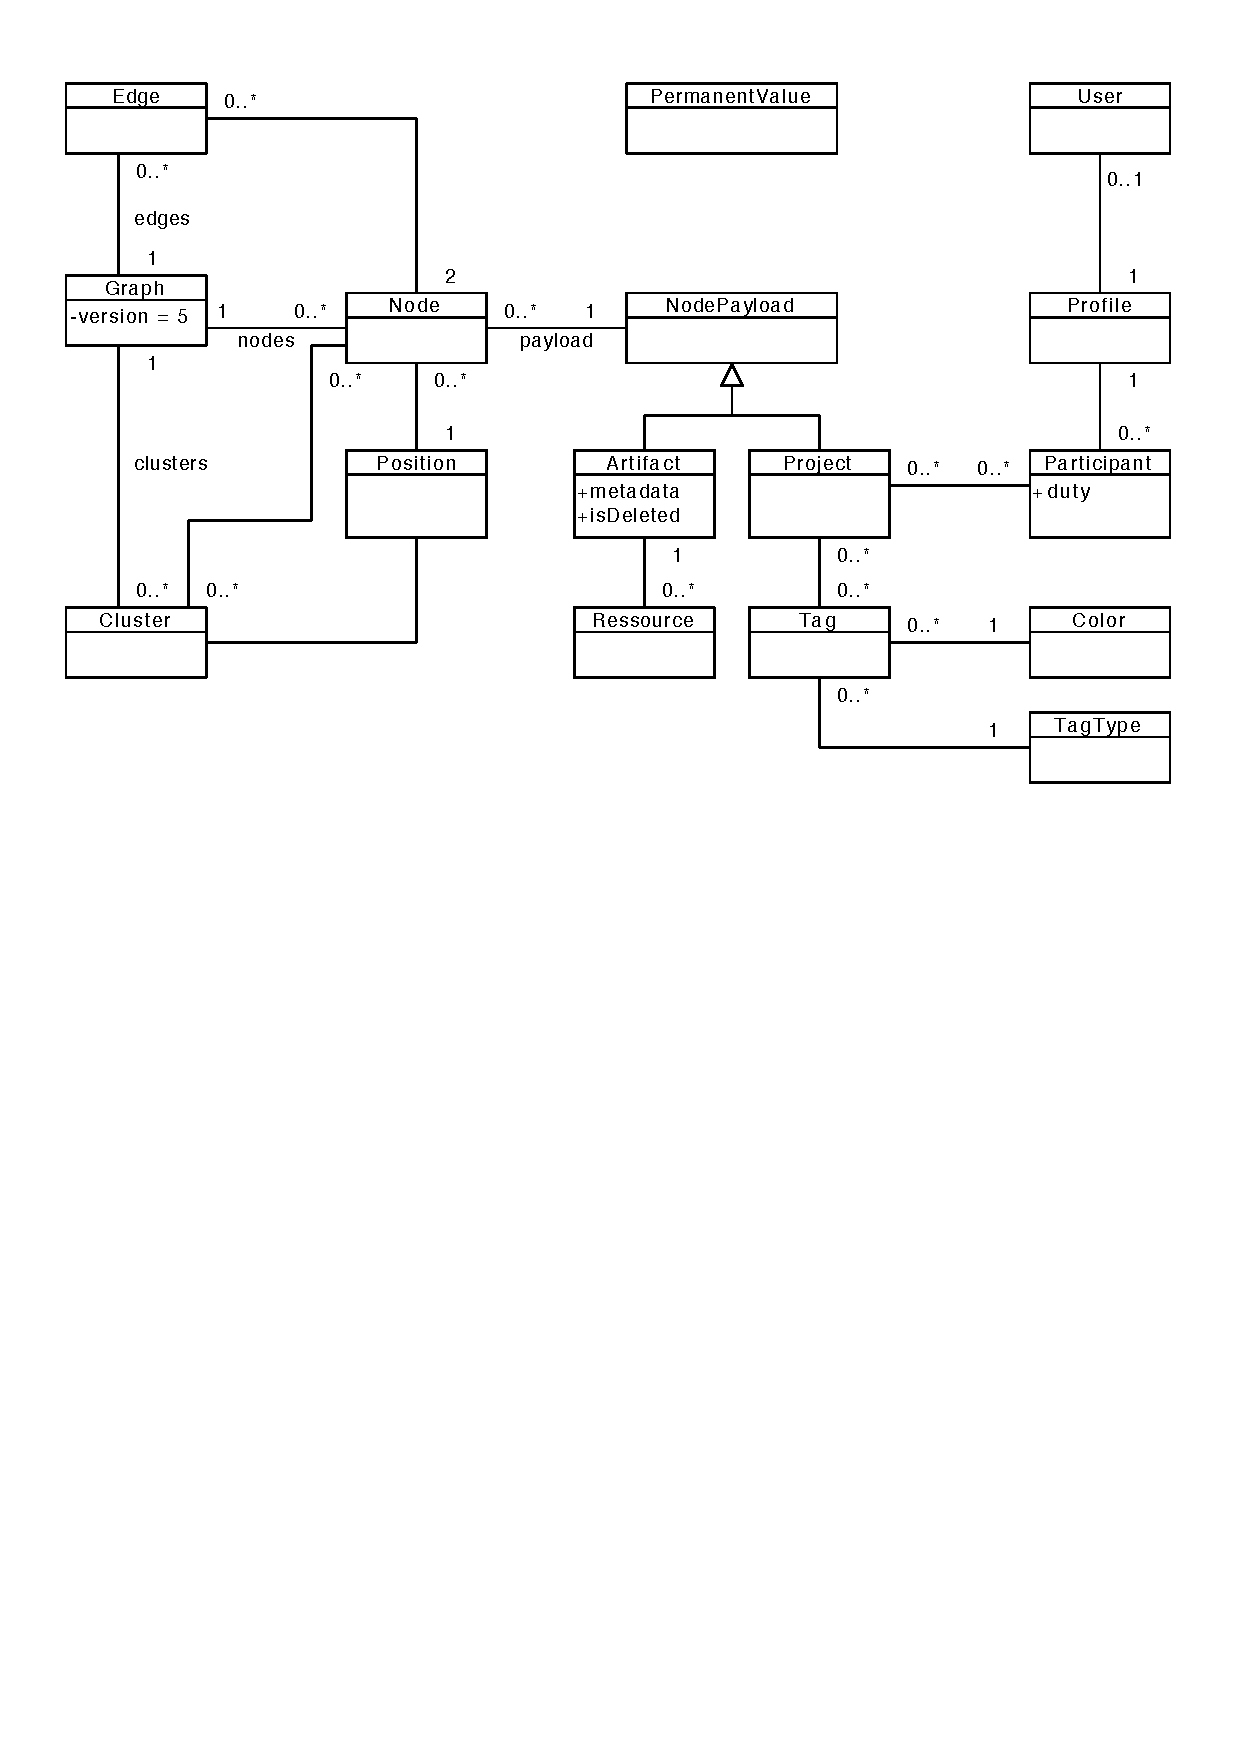
\includegraphics[width=1.0\textwidth]{img/complete_model.pdf}  
   \caption{Datenmodell von Project-Zoom}
  \label{fig:complete-model} 
\end{figure}

